% Beamer template
% Author: Ozgur Taylan TURAN
% Delft University of Technology

\documentclass[aspectratio=169]{beamer}
% PACKAGES
\usepackage[english]{babel}
\usepackage{graphicx}
\usepackage{animate}
%\usepackage{calc}
\usepackage{calligra}
\usepackage[absolute,overlay]{textpos}
\usepackage[T1]{fontenc}
%\usefonttheme{serif}
\usefonttheme{professionalfonts}
\usepackage{amsmath}
\usepackage{palatino}
\usepackage{mathpazo}
\usepackage{graphicx}
%\usepackage{subfig}
\usepackage{tikz}
\usepackage{ctable}
\usetikzlibrary{shapes,arrows}
\usepackage{xcolor}
\usepackage[T1]{fontenc}
%\usefonttheme{serif}
%\usepackage{titling}
\usepackage{graphicx}
%\usepackage{subfig}
%\usepackage{tikz}
%\usetikzlibrary{shapes,arrows}
\usepackage{mathtools}
\usepackage{cancel}
% CUSTOM PACKAGES
\usepackage{/home/taylanot/texmf/tex/beamerthemetot}
\input{/home/taylanot/texmf/presentation/tune.tex}

% COVER PAGE INFO   
\newcommand{\mytitle}{\color{White}\huge{\textbf{Coffee Talk \#8}}}
\newcommand{\mysubtitle}{\color{Pink}\Large{\textbf{Benign, Tempered or Catastrophic: A Taxonomy of Overfitting}}}
\newcommand{\myauthor}{\color{White}\textcalligra{\LARGE Ozgur Taylan Turan}}
\newcommand{\authorlabel}{\small O.T. Turan}
\author{\authorlabel}

\newcommand{\R}{\mathbb{R}}
\newcommand{\E}{\mathbb{E}}
\newcommand{\D}{\mathcal{D}}
\newcommand{\A}{\mathcal{A}}
\DeclareMathOperator*{\argmin}{arg\,min}
\begin{document}
% COVER PAGE

{
\def\beamer@entrycode{\vspace*{-\headheight}}
\setbeamertemplate{frametitle}[default][center]
\setbeamertemplate{navigation symbols}{}
\usebackgroundtemplate{
\includegraphics[width=\paperwidth,height=\paperheight]{cover/coverart.pdf}}

\begin{frame}[plain] 

\begin{minipage}{\textwidth}
	\centering{\mytitle} \\
	%\vspace{1cm}
	%\centering{\mysubtitle} \\
	\vspace{1cm}
	\centering{\color{White}November 15, 2021} \\
	\vspace{1cm}
	\centering{\myauthor}\\
\end{minipage}
\end{frame}
}


\begin{frame}
  \centering
  \mysubtitle\cite{mallinar2022}
\end{frame}

\begin{frame}{Why this paper?}
  \centering
  \begin{itemize}
    \item Discussion revolving around overfitting in one of the PR-Lab meetings.
  \end{itemize}
\end{frame}

\begin{frame}{Aim}
  \centering
  \begin{itemize}
    \item To create a taxonomy of overfitting for interpolating methods!
    \item To show \textit{overfitting} does not necessarily a good or a bad thing!
  \end{itemize}
\end{frame}

\begin{frame}{Introduction-A}
  \begin{minipage}{0.5\textwidth}
    \color{Pink} Classical statistical learning theory vs Double Descent
    \begin{itemize}
      \item Double Descent and Benign overfitting
    \end{itemize}
  \end{minipage}%
  \begin{minipage}{0.5\textwidth}
   % Bias-Variance Figure 
    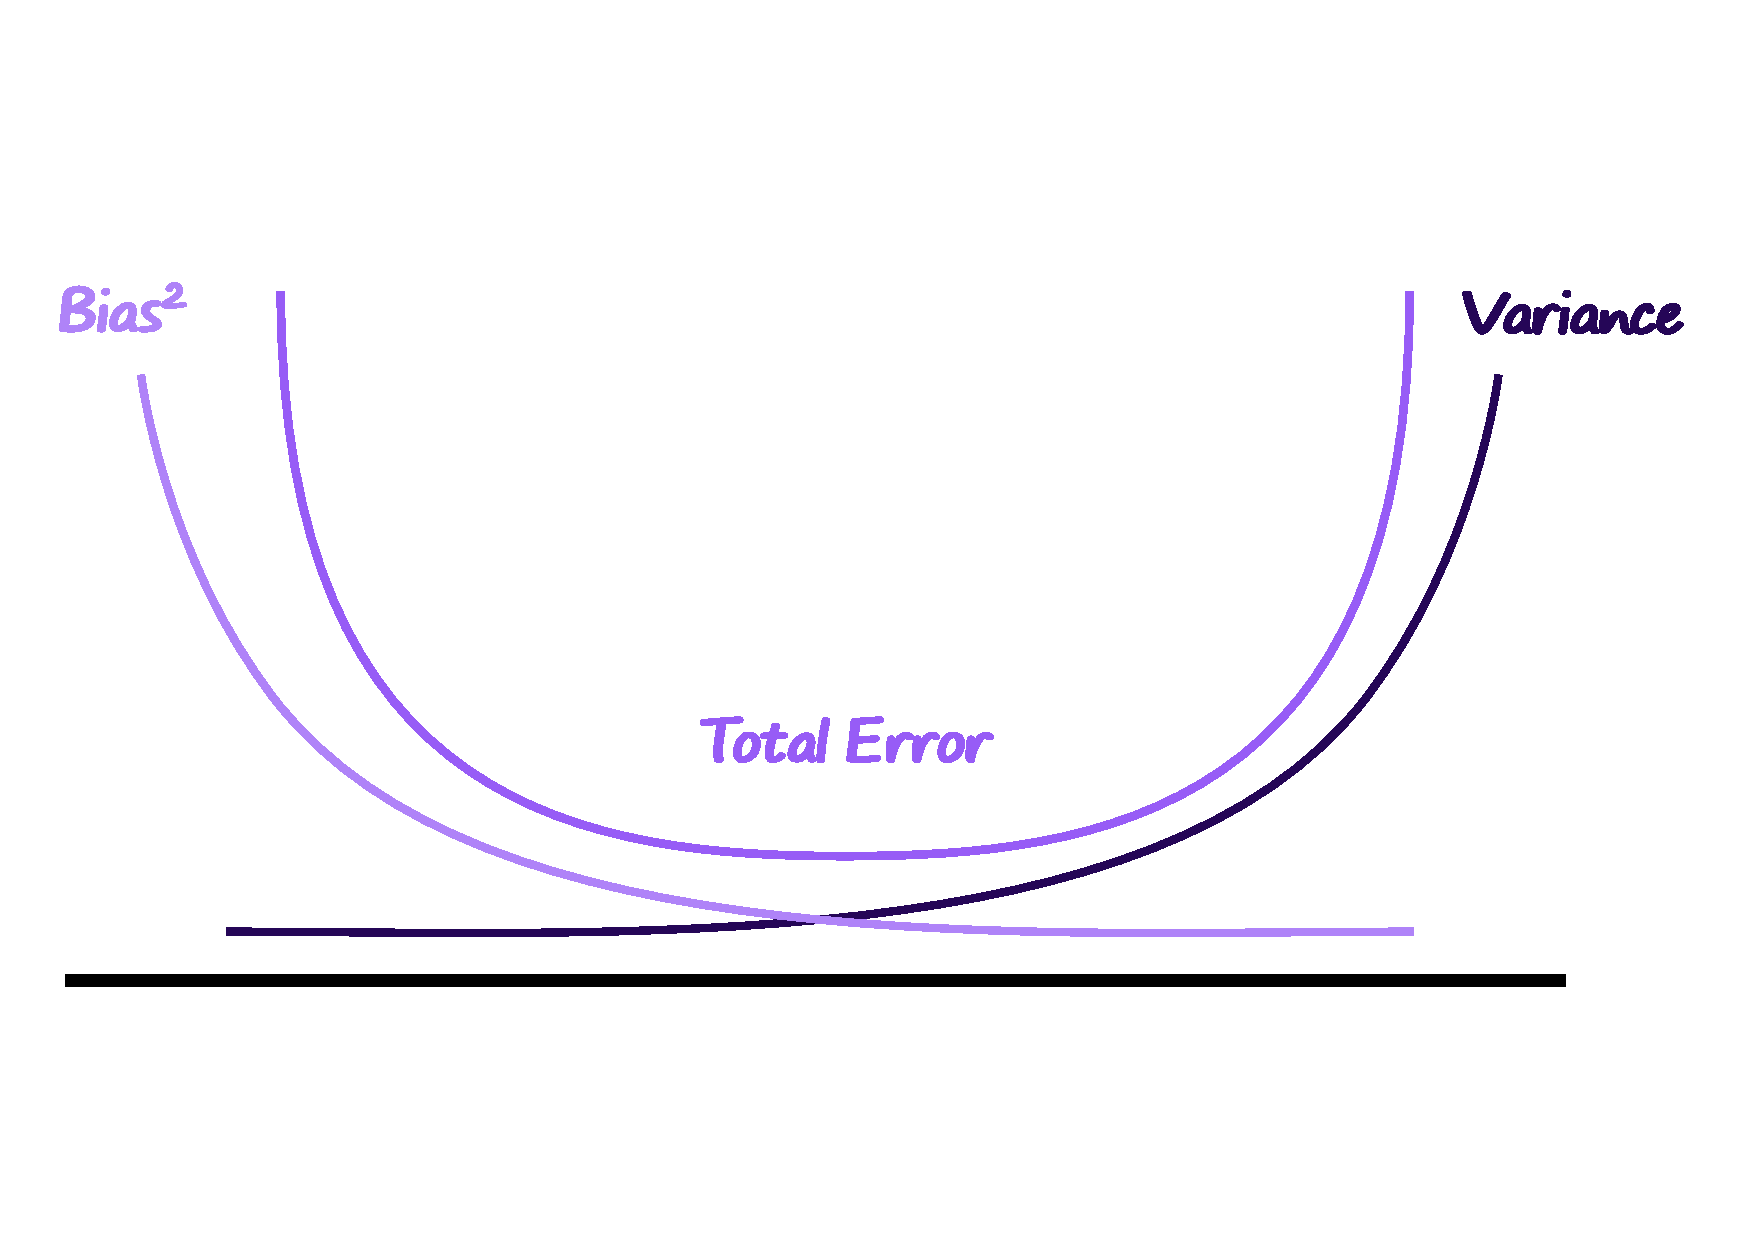
\includegraphics[width=\textwidth]{Figures/bias_variance}
  \end{minipage}
\end{frame}

\begin{frame}{Introduction-B}
  \begin{minipage}{\textwidth}
    \centering
    \color{Pink} Overfitting: \color{Black} fitting exactly to your training data. 

    \color{Pink} Interpolation $\sim$ Overfitting (in Belkin's works!)\color{Black}
  \end{minipage}
  \begin{minipage}{\textwidth}
   % Overfitting Types
    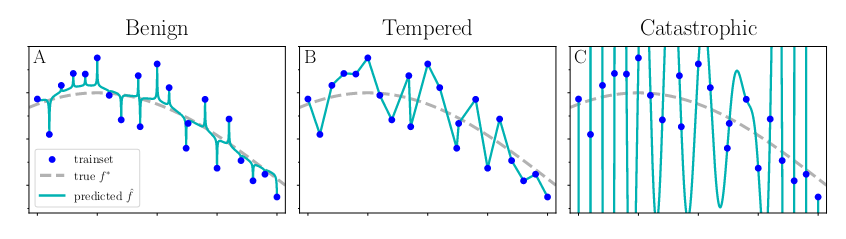
\includegraphics[width=\textwidth]{Figures/overfitting_types}
  \end{minipage}
\end{frame}

\begin{frame}{Problem Setting}
  \begin{minipage}{0.5\textwidth}
    % Until Excess Risk You have to give!
    \begin{itemize}
      \item Interpolation $:=$ Zero Training Error
      \item $\hat{f}:\mathcal{X}\to\R$ from $\mathcal{D}:=\{(x_i,y_i)\}_{i=1}^n$
      \item $\text{Var}[y_i|x_i] > 0$  \color{Pink} Non zero target noise! \color{Black}
    \end{itemize}
  \end{minipage}%
  \begin{minipage}{0.5\textwidth}
    \begin{itemize}
      \item Generalization performance $\mathcal{R}(\hat{f}):=\E_\D[(\hat{f}(x)-y)^2]$
      \item Bayes optimal solution: $f^*=\argmin_f R(f)$ gives the risk $R^*$
    \end{itemize}
  \end{minipage}
\end{frame}

\begin{frame}{Problem Setting-Learning Procedures}
  \only<1>
  {
  \begin{minipage}{0.5\textwidth}
     \color{Pink} Learning Procedure \color{Black}
    \begin{itemize}
      \item $\A:=\{\A_n\}_n$ are potentially stochastic functions 
      \item $\A_n:\D_n\to\hat{f}$ are potentially stochastic functions 
      \item \color{Pink} Risk of a Learning Procdure:

      \centering
      $R_n:=\E_{\A_n,\D_n}[R(\A_n(\D_n))]$
    \end{itemize}
    
  \end{minipage}%
  \begin{minipage}{0.5\textwidth}
    \centering
    \begin{tabular}{cc}
      \hline
      Benign        & $\lim_{n\to\infty}R_n=R^*$ \\
      Tempered      & $\lim_{n\to\infty}R_n\in(R^*,\infty)$ \\
      Catastrophic  & $\lim_{n\to\infty}R_n=\infty$ \\
      \hline
    \end{tabular}
  \end{minipage}
  }
  \only<2>
  {
  \begin{minipage}{\textwidth}
    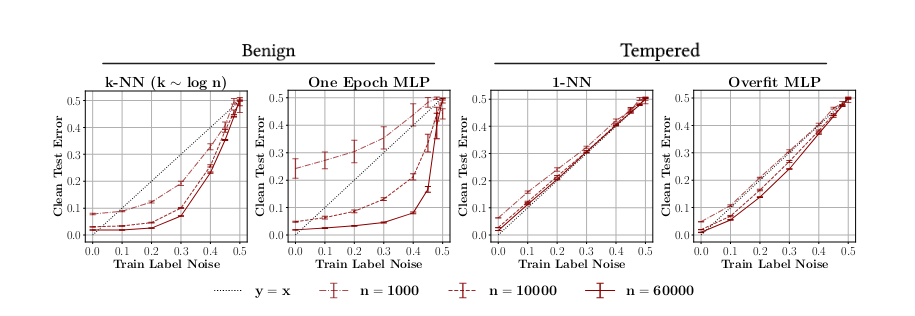
\includegraphics[width=\textwidth]{Figures/noise_profiles}
  \end{minipage}
  \begin{minipage}{\textwidth}
    \centering
    \begin{tabular}{cc}
      \hline
      Benign        & $\lim_{n\to\infty}R_n=R^*$ \\
      Tempered      & $\lim_{n\to\infty}R_n\in(R^*,\infty)$ \\
      Catastrophic  & $\lim_{n\to\infty}R_n=\infty$ \\
      \hline
    \end{tabular}
  \end{minipage}
  }
\end{frame}

\begin{frame}{Overfitting-Kernel Regression-A}
  \begin{minipage}{0.5\textwidth}
    \color{Pink} Neural Tangent Kernel (NTK)\cite{jacot2020a}: \color{Black} infinite width and time limit NNs with converge to "Ridless" ($\lambda=0$) Kernel Ridge Regression for Least Squares problem! 
    \color{Pink} NTK opens up a path for understanding the generalization of NNs.
  \end{minipage}%
  \begin{minipage}{0.5\textwidth}
    % Formulation of Kernel Ridge
    \centering
    $\hat{f}(x) = K(x,\mathbf{X})(K(\mathbf{X},\mathbf{X})+\delta\mathbf{I})^{-1}\mathbf{Y}$
  \end{minipage} 

\end{frame}

\begin{frame}{Overfitting-Kernel Regression-B}
  \begin{minipage}{\textwidth}
    % Give General Findings
    \only<1>
    {
    \begin{itemize}
      \item Exploiting $\E_{x^\prime}[K(x,x^\prime)\phi_i(x^\prime)]=\lambda_i\phi_i(x)$ and $\E_x[\phi_i(x)\phi_j(x)] = \delta_{ij}$
    \end{itemize}
    After some math\cite{simon2022} $R_n$ can be approximated by \textit{Modewise Learnabilities}:
    }
    \begin{itemize}
      \item A positive Ridge parameter or slow eigendecay $\to$ \textbf{Benign Overfitting}
      \item Powerlaw decay of eigenvalues $\to$ \textbf{Tempered Overfitting}
      \item Any decay faster than power law $\to$ \textbf{Catastrophic Overfitting} 
    \end{itemize}
  \end{minipage}
  \begin{minipage}{\textwidth}
    % Figures 
    \centering
  \includegraphics<2>[width=0.9\textwidth]{Figures/kernel_ridge.png}
  \end{minipage} 
\end{frame}

\begin{frame}{What do they do more?}
  \centering
  \begin{itemize}
    \item Computer vision examples showing tempered overfitting for interpolating ANNs.
    \item MLP on synthetic data: first benign, then tempered overfitting.
  \end{itemize}
\end{frame}

\begin{frame}{Conclusions}
  \centering
  \begin{itemize}
    \item Chill-out it! There is small chance that overfitting will hurt in modern applications of interpolating models?!
  \end{itemize}
  % Include Graphics here! 
  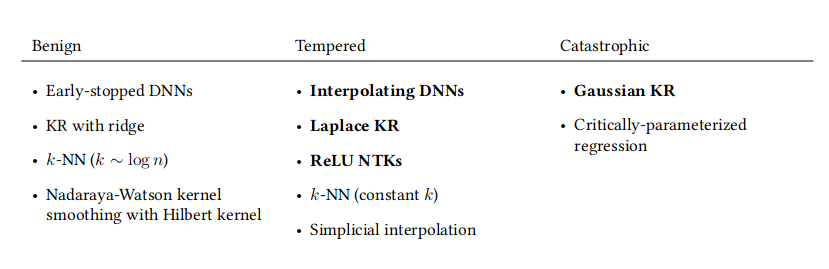
\includegraphics[width=\textwidth]{Figures/conclusions.png}
\end{frame}

\begin{frame}
    \color{Pink} 
    \centering
     THANKS!
\end{frame}


\end{document}

